
\section{Introduction}

Programs in higher-order languages heavily use function calls and method dispatch as part of their control flow.
%
Until recently, flow analyses for higher-order languages could not handle return flow precisely \citep{ianjohnson:vardoulakis-lmcs11, dvanhorn:Earl2010Pushdown}, which leads to several spurious paths (and thus false positives) due to the pervasiveness of function or method calls and subsequent returns.
%
These works, called CFA2 and PDCFA respectively, use pushdown automata as their approximation's target model of computation.
%
They are hence called ``pushdown analyses.''
%
\footnote{We will refer to the classic finite model analyses as ``regular analyses'' after regular languages.}
%
CFA2 and PDCFA have difficult details to easily apply to an off-the-shelf semantics --- especially if they feature non-local control transfer that breaks the pushdown model.
%%

%%
There is a systematic process for transforming off-the-shelf programming language semantics into a form amenable to \emph{regular} analysis that has been widely applied with great success to production programming languages~\citet{dvanhorn:VanHorn2010Abstracting} (a technique called abstracting abstract machines, or AAM).
%
A contribution of this paper is a systematic process to construct \emph{pushdown} analyses of programming languages, due to the precision (and often performance) benefits.
%

%%

%%
Testing new ideas in analysis for improving precision or increasing performance can be a difficult venture.
%
We contend that the machinery that we employ in the abstract should have a concrete counterpart that maintains the meaning of the language so that we can see their effect without introducing approximations which might mask correctness issues.
%
Abstraction should be a simple process that is ``obviously correct.''
%
The framework we present in this paper is applicable in the concrete such that a point-wise abstraction leads to the pushdown analyses in the literature.
%%

%%
This paper gives a common, simple framework to derive CFA2, PDCFA and its garbage-collecting extension using a recipe to apply pushdown analysis techniques to arbitrary semantics in a manner similar to AAM.
%
To exercise the recipe further, we give a novel analysis for delimited, composable control. \\

\section{The essence of summarization}

CFA2 uses a technique called ``summarization'' from Sharir and Pnueli \citep[Chapter 7]{local:muchnick:jones:flow-analysis:1981}, which is synonymous with the $\epsilon$-closure graph that PDCFA constructs.
%
Summarization algorithms need not be restricted to languages with well-bracketed calls and returns.
%
We can adopt the technique for higher precision in the common case but still handle difficult cases such as first-class control.
%
This was shown for the \rackett{call-with-current-continuation} (a.k.a. \rackett{call/cc}) operator in ~\citet{ianjohnson:Vardoulakis2011Pushdown}.
%
This impressive work illuminated the fact that we can harness the enhanced technology of pushdown analyses in non-pushdown models of computation.
%
Doing this sacrifices call/return matching in the general case, but in practice the precision is much better than the alternative regular model that, say, 0-CFA would provide.
%%

%%
A downside of the work providing \rackett{call/cc} is that it was an algorithmic change to the already complicated CFA2 --- there was no recipe for how to do this for one's favorite control operator.
%
This paper seeks to do just that with an operational view of what summarization is, in essence.
%
In other words, we give a concrete semantics to the tricks that the analyses in the literature use in the abstract, and maintain the original meaning of the language.
%
We also give intuitive analogies to well-established ideas and techniques so that the working semanticist can write a pushdown analysis for her language.
%
In order to demonstrate the applicability of this viewpoint, we show a new analysis for a language with composable control.
%
All of the semantics modeled in this paper are implemented in full detail in PLT Redex~\citep{ianjohnson:Felleisen:2009:SEP:1795772} and available online\footnote{\url{http://github.com/ianj/concrete-summaries}}.

There are common underpinnings of PDCFA and CFA2 that can be embodied as concrete ``summarization'' machinery in the programming language semantics: 
\begin{enumerate}
\item{bound continuations with with delimiters that specify the exact context in which any continuation replacement would lead to the same result, and}
\item{memoize at these delimiters}
\end{enumerate}

%%
The first of these two might seem unfamiliar, but it is just identifying what is needed for sound memoization, and we delimit the continuations in order to mark where to memoize results.
%
In the case of a CESK machine, where the store is relevant to the evaluation of functions, a context is just the CES portion since stacks don't matter.
%
For stack inspecting analyses, a context is CES plus the inspected portion of K.
%
As soon as we have a value that such a context evaluates to, all subsequent visits to that context can jump straight to the memoized result(s).
%%

%%
Once the machine semantics is in this form, simple point-wise abstraction leads to the summarization algorithms that we see in the literature.
%
In \autoref{sec:pdcfa} we derive a cousin of PDCFA.
%
The following section shows how to extend PDCFA with abstract garbage collection. % \autoref{sec:gc}: we show how abstract garbage collection ``falls out'' of this approach.
%
Then in \autoref{sec:cfa2} we show the fundamental difference between PDCFA and CFA2 without first-class control. % : we make additions to the PDCFA semantics to get a direct-style CFA2 without first-class control}
%
\ifwcm{We show in \autoref{sec:wcm} that semantics with stack-inspection (beyond GC) also fit within this interpretation.}
%
Finally, we show in \autoref{sec:sr} that even though first-class control operators don't fit in the pushdown model, we can gracefully loosen the abstraction to analyze delimited, composable first-class control.

\section{Deriving PDCFA}
\label{sec:pdcfa}

PDCFA does not have some orthogonal semantic components that CFA2 features to improve precision and is thus the simpler of the two.
%
The key to their method is to notice in languages without stack-capturing features, the continuation is only modified a frame at a time.
%
If the state space without the stack is finite (and it can be made finite with an approximation ala AAM), then the model falls directly into the realm of pushdown systems.
%
They thus recast the problem in terms of pushdown systems.
%
The whole of their machinery is then computing the pushdown system on-the-fly, only considering states reachable from the initial state.
%
They call the main data-structure for this a Dyck state graph.
%
They additionally compute an $\epsilon$-closure graph to match nodes that push frames with later nodes following the pop of that frame, which keeps edges between nodes that have a net-zero stack change path between them.
%
We skip the detour to pushdown systems altogether and show an operational understanding of the resulting analysis.
%%

%%
We start by deriving PDCFA from an operational semantics for the untyped lambda calculus (\autoref{fig:base-semantics}).
%
The semantic spaces for the machine follow.

{
\setlength{\abovedisplayskip}{0pt}
\setlength{\belowdisplayskip}{4pt}
\setlength{\abovedisplayshortskip}{0pt}
\setlength{\belowdisplayshortskip}{8pt}
\begin{align*}
  \mexpr \in \Expr = \svar{\mvar} \alt \sapp{\mexpr}{\mexpr} \alt \slam{\mvar}{\mexpr}
\end{align*}
\begin{minipage}[b]{.55\linewidth}
  \begin{align*}
  \mstate \in \State &= (\Expr \times \Env) \times \Store \times \Kont \\
  \mval \in \Value &::= \vclo{\slam{\mvar}{\mexpr}}{\menv} \\
  \mkont \in \Kont &::= \kmt \alt \kcons{\mkframe}{\mkont} \\
  \mkframe \in \Frame &::= \kar{\mexpr,\menv} \alt \kfn{\mval}
  \end{align*}\hrule height 0pt\end{minipage}
\begin{minipage}[b]{.40\linewidth}
  \begin{align*}
  \menv \in \Env &= \Var \to \Addr \\
  \mstore \in \Store &= \Addr \to \wp(\Value) \\
  \mvar \in \Var &\text{ an infinite set} \\
  \maddr \in \Addr &\text{ an infinite set}
  \end{align*}\hrule height 0pt\end{minipage}
}
%%

%%
The $\Addr$ space is what controls the precision of the model.
%
For a concrete semantics, we require the allocation meta-function $\alloc :
\State \to \Addr$ to return fresh addresses ($\alloc(\mstate) \notin \dom(\mstate.\mstore)$), but any choice of address is sound~\citep{dvanhorn:Might2009Posteriori}.
%
If $\alloc$ only uses addresses from a finite subset of $\Addr$, then the state space without continuations is finite, and the space of contination frames is finite --- thus the pushdown system interpretation is apt.
%
This meta-function along with the commitment to having no recursive data-structures is the key to the AAM technique.
%
All recursion can be expressed by indirecting through addresses into a store --- tying Landin's knot.
%
We borrow this technique on top of our own.

\begin{figure}
  \centering
  $\mstate \stepto \mstate' \text{ where } \maddr = \alloc(\mstate)$ \\
  \begin{tabular}{r|l}
    \hline
% variable lookup
    $\tpl{(\svar\mvar, \menv), \mstore, \mkont}$
    &
    $\tpl{\mval,\mstore,\mkont}$ if $\mval \in \mstore(\menv(\mvar))$
    \\
% application
    $\tpl{(\sapp{\mexpri0}{\mexpri1}, \menv), \mstore, \mkont}$
    &
    $\tpl{(\mexpri0, \menv), \mstore, \kcons{\kar{\mexpri1,\menv}}{\mkont}}$
    \\
% argument evaluation
    $\tpl{\mval, \mstore, \kcons{\kar{\mexpr,\menv}}{\mkont}}$
    &
    $\tpl{(\mexpr, \menv), \mstore, \kcons{\kfn{\mval}}{\mkont}}$
    \\
% function call
    $\tpl{\mval,\mstore,\kcons{\kfn{\vclo{\slam{\mvar}{\mexpr}}{\menv}}}{\mkont}}$
    &
    $\tpl{(\mexpr, \extm{\menv}{\mvar}{\maddr}), \joinone{\mstore}{\maddr}{\mval}, \mkont}$
  \end{tabular}
  \caption{The CESK machine with allocation tuning}
  \label{fig:base-semantics}
\end{figure}

\paragraph{Tracking return points:} the magic of the method is in keeping a table of continuation segments for each function and store pair, where the continuation is segmented at function boundaries.
%
This closely mirrors the technique of store-allocating continuations used in AAM.
%
Instead of deferring to the table (store) for the remainder of a continuation for each frame, we only have indirections at function call boundaries (see rules 4 and 5 in figure \ref{fig:summary-semantics} for saving and restoring continuations).
%
Note that since AAM is about finitizing the state space, this step itself fits within the AAM method, since continuations within functions truncated at call boundaries are bounded by the nesting depth of those functions, thereby making the continuation space finite.
%
In the monovariant case, the number of continuations is still linear in the size of the program.
%%

%%
The tail of a continuation in the context of a function will contain the stack-less context in which the function was called, in order to link up with the proper call-site(s).
%
The context includes the function (or unique label of the function), the environment, and the store.
%
Notice that this choice can be viewed as a special allocation strategy for continuations in the AAM viewpoint, but we separate the table of continuations from the store since continuations themselves contain stores in $\rt$ continuations --- this leads to a recursive data-structure that we are trying to avoid.
%
The store is an important ingredient to maintaining enough precision to keep a pushdown abstraction.
%
The semantic spaces for the machine are modified thusly:

\begin{align*}
  \mstate \in \State &= (\Expr \times \Env) \times \Store \times \Kont \times \KTab \times \Memo \\
  \mkont \in \Kont &::= \kmt \alt \krt{(\mexpr,\menv),\mstore} \alt \kcons{\mkframe}{\mkont} \\
  \mktab \in \KTab &= (\Expr \times \Env)\times \Store \to \wp(\Kont) \\
  \mmemo \in \Memo &= (\Expr \times \Env)\times \Store \to \wp(\Value \times \Store)
\end{align*}

\paragraph{The role of summaries:} notice the additional $\Memo$ component.
%
A ``summary edge'' in CFA2 or equivalently an $\epsilon$-edge in PDCFA is an edge from the source of a push edge to the target of the matching pop edge.
%
``Matching'' here means there is a path through machine reductions that don't change the stack, or through summary edges.
%
In our model, we only ``push'' when we call a function, and we only ``pop'' when we return with a value.
%
There is an analogy to something more operational: summary edges embody memoization (see the last rule in figure \ref{fig:summary-semantics}).
%
Instead of following an entire path through a call to return a value, we simply jump from the call to the return with the result of the call, with the resulting context changes---in this case only the store (the second case of rule 4).
%%

%%
Memoization with respect to the entire store is safe, if not a little wasteful; there are portions of the store that can change and be irrelevant to the result of a function call.
%
There are techniques to ignore differences in the heap when they are irrelevant, dubbed ``sparseness analysis'' that have been successful for large-scale first-order analysis~\citep{ianjohnson:DBLP:conf/pldi/OhHLLY12}, but they rely on a pre-analysis that knows the control-flow graph.
%
We have promising preliminary results in this direction that don't require a pre-analysis, but we leave further investigation of sparse techniques to future work.

\begin{figure}
  \centering
  $\mstate \stepto \mstate' \text{ where } \maddr = \alloc(\mstate)$ \\
  \begin{tabular}{r|l}
    \hline
% variable lookup
    $\tpl{(\svar\mvar, \menv), \mstore, \mkont, \mktab, \mmemo}$
    &
    $\tpl{\mval,\mstore,\mkont, \mktab, \mmemo}$ if $\mval \in \mstore(\menv(\mvar))$
    \\
% application
    $\tpl{(\sapp{\mexpri0}{\mexpri1}, \menv), \mstore, \mkont, \mktab, \mmemo}$
    &
    $\tpl{(\mexpri0, \menv), \mstore, \kcons{\kar{\mexpri1,\menv}}{\mkont}, \mktab, \mmemo}$
    \\
% argument evaluation
    $\tpl{\mval, \mstore, \kcons{\kar{\mexpr,\menv}}{\mkont}, \mktab, \mmemo}$
    &
    $\tpl{(\mexpr, \menv), \mstore, \kcons{\kfn{\mval}}{\mkont}, \mktab, \mmemo}$
    \\
% function call
    $\tpl{\mval,\mstore,\kcons{\kfn{\vclo{\slam{\mvar}{\mexpr}}{\menv}}}{\mkont},\mktab,\mmemo}$
    & % actually do call,
    $\tpl{\mpoint,
          \mstore',
          \krt{\mpoint, \mstore'},
          \mktab',
          \mmemo}$
\\
    & or \\
    & $\tpl{\mval_\mathit{result},
            \mstore'',
            \mkont,
            \mktab',
            \mmemo}$
    \\ & \quad if $(\mval_\mathit{result},\mstore'') \in \mmemo(\mpoint,\mstore')$
    \\ % or, lookup in table
%    & $\tpl{\mval, \mstore', \mkont,\mktab,\mmemo}$ if $\mval \in \mmemo(\mpoint, \mstore')$ \\    
    where & $\mpoint = (\mexpr, \extm{\menv}{\mvar}{\maddr})$ \\
          & $\mstore' = \joinone{\mstore}{\maddr}{\mval}$ \\
          & $\mktab' = \joinone{\mktab}{(\mpoint, \mstore')}{\mkont}$
    \\
% return
    $\tpl{\mval, \mstore, \krt{\mpoint,\mstore'}, \mktab, \mmemo}$
    &
    $\tpl{\mval, \mstore, \mkont, \mktab, \joinone{\mmemo}{(\mpoint, \mstore')}{(\mval,\mstore)}}$
    \\ & \quad if $\mkont \in \mktab(\mpoint, \mstore')$
  \end{tabular}
  \caption{The summarizing tabular stack machine}
  \label{fig:summary-semantics}
\end{figure}

To turn this semantics into PDCFA's algorithm for constructing a Dyck state graph, given the appropriate $\alloc$, we apply a widening operator to make $\mstore$, $\mkont$, and $\mmemo$ shared amongst all states (meaning states then become represented without these components), in what is then called a $\System$. We use a meta-function $\wn$, ``wide to narrow,'' to shift between the two representations of states.
%%

%%
We show only the memo and continuation table widening, since store widening would require rewriting newly-created contexts to use the global store following the step.
%
This rewriting is unnecessary with the store-counting per-wide-step technique presented in \citet{ianjohnson:oaam:icfp2013}, or the less precise timestamp approximation from \citet{dvanhorn:Shivers:1991:CFA}.
%
Since these components are shared, they are always the least upper bound of any respective component that the semantics produces (the intermediate set $I$) in order to stay sound.

%% FIXME: remove stores from memo-table since they will always be unchanged
%% TODO: Show that store widening and store/memo/KTab widening have a bisimulation.
{
\setlength{\abovedisplayskip}{0pt}
\setlength{\belowdisplayskip}{4pt}
\setlength{\abovedisplayshortskip}{0pt}
\setlength{\belowdisplayshortskip}{8pt}
\begin{align*}
  \mastate \in \sa{State} &= (\Expr \times \Env) \times \Store \times \Kont \\
  \System &= \wp(\sa{State}) \times \wp(\sa{State}) \times \KTab \times \Memo \\
  {\mathcal F} &: \sa{\State} \to \System \to \System \\
  {\mathcal F}(\mastate_0)(S, F, \mktab, \mmemo) &= (S \cup S', F', \mktab', \mmemo') \\
  \text{where } I &= \setbuild{\mstate'}{\mastate \in F, \wn(\mastate,\mktab,\mmemo) \stepto \mstate'} \\
                \wn(\tpl{(\mexpr,\menv),\mstore,\mkont},\mktab,\mmemo)
                   &= \tpl{(\mexpr,\menv),\mstore,\mkont,\mktab,\mmemo}
\end{align*}
\begin{minipage}{.55\linewidth}
  \begin{align*}
    \mktab' &=  \bigsqcup\setbuild{\mktab'}{\wn(\_, \_, \mktab', \_) \in I} \\
    \mmemo' &= \bigsqcup\setbuild{\mmemo'}{\wn(\_, \_, \_, \mmemo') \in I}
  \end{align*}
\end{minipage}
\begin{minipage}{.40\linewidth}
  \begin{align*}
    S' &= \setbuild{\mastate'}{\wn(\mastate', \_, \_, \_) \in I} \cup \set{\mastate_0}\\
    F' &= S' \setminus S
  \end{align*}
\end{minipage}
}
%%

%%
A $\System$ embodies the states seen and at which store, $S$, the frontier set of states yet to analyze, $F$, the continuation table $\mktab$ and the memo table $\mmemo$.
% Note: Only if widened store.{
%
%The memo table need only map to values, since the global store will always subsume the store that would otherwise be mapped.
%
%All the states in the frontier are stepped with the current store, after which the next store is the least upper bound of all the resulting stores.
%
%The next frontier contains only states resulting from stepping the previous frontier that we haven't seen at this next store.}
%
The least fixed-point of ${\mathcal F}(\tpl{(\mexpr,\bot),\bot,\kmt})$ is the analysis of closed expression $\mexpr$.
%
Systematic techniques for a performant implementation can be found in \citet{ianjohnson:oaam:icfp2013}.

\paragraph{Example:} Let's consider a monovariant allocation strategy (the address for each binding is the variable name itself, so $\menv$ is always the identity function $\iota$) to run the following example:

\begin{center}
  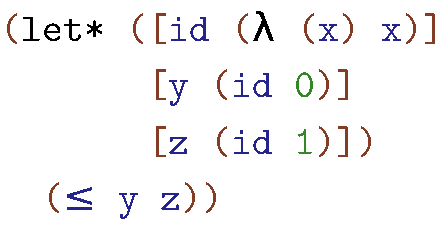
\includegraphics[scale=0.5]{example0}
\end{center}
  % \item{\texttt{(id 0)} steps to \texttt{x} at $\krt{((\texttt{x}, [\texttt{x}\mapsto\texttt{x}]), \mstore_0)}$ with $\mstore_1 =
%     \mstore_0[\texttt{x} \mapsto \set{0}]$ and
%     (let $\mctx_1 = ((\texttt{x},[\texttt{x}\mapsto\texttt{x}]),\mstore_1)$,
%          $\mkont_1 = \klet{\texttt{y}, \texttt{(let ([z (id 1)]) ($\le$ y z))}, [\texttt{id}\mapsto{\texttt{id}}]}$)
%     $\mktab_1 = [\mctx_0 \mapsto \set{\mkont_0}]$}
% \item{\texttt{0} at $\krt{\mctx_1}$ steps to $0$ at $\mkont_1$ and $\mmemo_1 = [\mctx_1 \mapsto \set{0}]$}
% \item{\texttt{0} at $\mkont_1$ steps to \texttt{(let ([z (id 1)]) ($\le$ y z))} and $\mstore_2 = \mstore_1[\texttt{y} \mapsto \set{0}]$}
% \item{\texttt{(let ([z (id 1)]) ($\le$ y z))} steps to \texttt{(id 1)} at \\
%       $\klet{\texttt{z}, \texttt{($\le$ y z)}, [\texttt{id} \mapsto \texttt{id}, \texttt{y} \mapsto \texttt{y}]}$
%       (call this $\mkont_2$).}
% \item{\texttt{(id 1)} steps to $x$ with $\mstore_3 = \mstore_2[\texttt{x} \mapsto \set{0,1}]$ and
%       (let $\mctx_3 = ((\texttt{x},[\texttt{x}\mapsto\texttt{x}]),\mstore_3)$) $\mktab_3 =\mktab_1[\mctx_3 \mapsto \set{\mkont_2}]$.}
% \item{\texttt{0} or \texttt{1} at $\krt{\mctx_3}$ steps to \texttt{0} or \texttt{1} at $\mkont_2$ and $\mmemo_3 = \mmemo_1[\mctx_3 \mapsto \set{0,1}]$.}
% \item{\texttt{z} gets bound to $\set{0,1}$, and \texttt{($\le$ y z)} evaluates to true.}


Suppose we extend our semantics to allow numbers, numeric primitives and \texttt{let}.
%
The continuation frame for a \texttt{let} contains the identifier to bind to the resulting value, along with the body of the \texttt{let} with its environment.
%
Call the constructor of this frame $\mathbf{lt}$.
%%

%%
We should expect that a pushdown analysis would predict this evaluates to true, and there are no loops in the program.
%
0CFA~\citep{dvanhorn:Shivers:1991:CFA} claims there is a loop from the second call of \texttt{id} to the first, and thusly predicts this program evaluates to true or false.
%
PDCFA claims there is no loop, and depending on the implementation, that the result is true or false (paper), or just true (implemented)
\footnote{This is because the paper steps every seen state with the current store every iteration, but the implementation only steps states that need stepping.}.
%
The example evaluation is in \autoref{fig:ex-eval}.
%
We maintain enough context to distinguish the return points of \texttt{id} to not rebind \texttt{y} to 1.
%
When determining control flow through the expression, we consult $\mmemo$ to continue past function calls, so there is no confusion about a back edge from the second call to \texttt{id}.
%

\begin{figure}
  \centering
    \begin{minipage}{0.55\linewidth}
      \begin{center}
        $\begin{array}{l}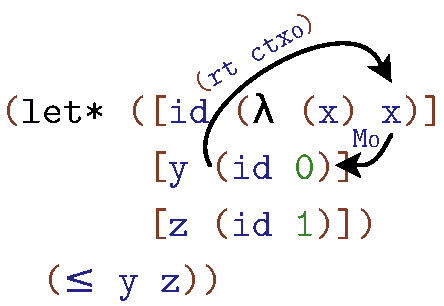
\includegraphics[scale=0.65]{example1}\end{array}$ \\
        $\Downarrow$ \\
        $\begin{array}{l}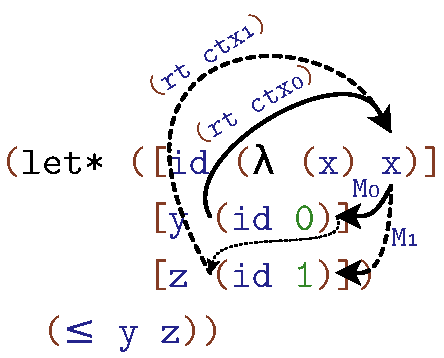
\includegraphics[scale=0.65]{example2}\end{array}$ \\
        $\Downarrow$ \\
        $\begin{array}{l}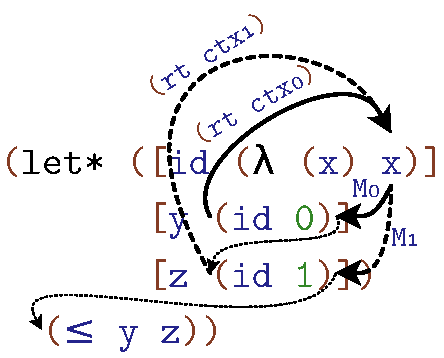
\includegraphics[scale=0.65]{example3}\end{array}$
      \end{center}
    \end{minipage}
    \begin{minipage}{0.43\linewidth}
      \begin{center} {\small
        \begin{tabular}{|l|c|c|}
          \hline
          \# & $\mstore$ & $\mkont$ \\
          \hline
          0 & $[{\tt id} \mapsto \set{(\slam{\mvar}{\mvar},\bot)}]$ & $\mkont_0$ \\
          1 & $\mstore_0[{\tt \mvar} \mapsto \set{0}]$ & $\krt{\mctx_0}$ \\
          2 & $\mstore_1[{\tt y} \mapsto \set{0}]$ & $\mathbf{lt}({\tt z}, {\tt (}\le\ {\tt y}\ {\tt z)})$ \\
          3 & $\mstore_2[{\tt x} \mapsto \set{0,1}]$ & $\krt{\mctx_1}$ \\
          4 & $\mstore_3[{\tt z} \mapsto \set{0,1}]$ & $\kmt$ \\
          \hline
        \end{tabular}} \\[10pt]
      {\small
        \begin{tabular}{|l|c|}
          \hline
          \# & $\mctx$ \\
          \hline
          0  & $(({\tt x}, \iota), \mstore_1)$ \\
          1  & $(({\tt x}, \iota), \mstore_3)$ \\
          \hline
        \end{tabular}}
      \\[10pt]
      {\small
        \begin{tabular}{|l|c|c|c|}
          \hline
          \# & $\mktab$ & $\mmemo$ \\
          \hline
          0  & $[\mctx_0 \mapsto \set{\mkont_0}]$ & $[\mctx_0 \mapsto \set{0}]$ \\
          1  & $\mktab_0[\mctx_1 \mapsto \set{\mkont_2}]$ & $\mmemo_0[\mctx_1 \mapsto \set{0,1}]$ \\
          \hline
        \end{tabular}}    
    \end{center}
  \end{minipage}
Where $\mkont_0 = \mathbf{lt}({\tt y}, {\tt (let\ ([z\ (id\ 1)])\ (}\le\ {\tt y}\ {\tt z))}, \iota)$
\caption{Example analysis evaluation}
\label{fig:ex-eval}
\end{figure}
% %% FIXME stores in memo-table
% \begin{enumerate}
% \item{\texttt{(id 0)} steps to \texttt{x} at $\krt{((\texttt{x}, [\texttt{x}\mapsto\texttt{x}]), \mstore_0)}$ with $\mstore_1 =
%     \mstore_0[\texttt{x} \mapsto \set{0}]$ and
%     (let $\mctx_1 = ((\texttt{x},[\texttt{x}\mapsto\texttt{x}]),\mstore_1)$,
%          $\mkont_1 = \klet{\texttt{y}, \texttt{(let ([z (id 1)]) ($\le$ y z))}, [\texttt{id}\mapsto{\texttt{id}}]}$)
%     $\mktab_1 = [\mctx_0 \mapsto \set{\mkont_0}]$}
% \item{\texttt{0} at $\krt{\mctx_1}$ steps to $0$ at $\mkont_1$ and $\mmemo_1 = [\mctx_1 \mapsto \set{0}]$}
% \item{\texttt{0} at $\mkont_1$ steps to \texttt{(let ([z (id 1)]) ($\le$ y z))} and $\mstore_2 = \mstore_1[\texttt{y} \mapsto \set{0}]$}
% \item{\texttt{(let ([z (id 1)]) ($\le$ y z))} steps to \texttt{(id 1)} at \\
%       $\klet{\texttt{z}, \texttt{($\le$ y z)}, [\texttt{id} \mapsto \texttt{id}, \texttt{y} \mapsto \texttt{y}]}$
%       (call this $\mkont_2$).}
% \item{\texttt{(id 1)} steps to $x$ with $\mstore_3 = \mstore_2[\texttt{x} \mapsto \set{0,1}]$ and
%       (let $\mctx_3 = ((\texttt{x},[\texttt{x}\mapsto\texttt{x}]),\mstore_3)$) $\mktab_3 =\mktab_1[\mctx_3 \mapsto \set{\mkont_2}]$.}
% \item{\texttt{0} or \texttt{1} at $\krt{\mctx_3}$ steps to \texttt{0} or \texttt{1} at $\mkont_2$ and $\mmemo_3 = \mmemo_1[\mctx_3 \mapsto \set{0,1}]$.}
% \item{\texttt{z} gets bound to $\set{0,1}$, and \texttt{($\le$ y z)} evaluates to true.}
% \end{enumerate}

\begin{theorem}\label{thm:pdcfa-tabular}
  Tabular semantics has a bisimulation with the standard semantics with comparable allocation strategies.
\end{theorem}

This follows directly from the invariants we prove of $\mktab$ and $\mmemo$ in the tabular semantics.
%
Allocation strategies are comparable if they produce equal addresses regardless of the differences in the state representations.
%
More formally, $\alloc$ and $\alloc^*$ are comparable if this implication holds:
\begin{mathpar}
  \inferrule{\mkont \in \unroll{\mktab}{\mkont^*}}
            {\alloc(\tpl{\mpoint,\mstore,\mkont}) = \alloc^*(\tpl{\mpoint,\mstore,\mkont^*,\mktab,\mmemo})}
\end{mathpar}

The $\mathit{unroll}$ function interprets what are all the valid continuations that $\mktab$ encodes for a given continuation that contains $\krt{\mctx}$, defined as the greatest fixed point of the following rules:
\begin{mathpar}
  \inferrule{ }{\kmt \in \unroll{\mktab}{\kmt, G}} \quad
  \inferrule{\mkont \in \unroll{\mktab}{\mkont', \emptyset}}{\mkframe:\mkont \in \unroll{\mktab}{\mkframe:\mkont', G}} \\
  \inferrule{\mctx \notin G  \\
             \mkont^\circ \in \mktab(\mctx) \\
             \mkont \in \unroll{\mktab}{\mkont^\circ, \set{\mctx}\cup G}}
            {\mkont \in \unroll{\mktab}{\krt{\mctx}, G}}  
\end{mathpar}

We add $G$ to protect against unguarded corecursion in order for the definition to be well-defined.
%
Interpreting a function with ill-founded recursion can lead to a table such that $\krt{\mctx} \in \mktab(\mctx)$.
%
The abstractions that we impose on our data might also cause this situation, even though the concrete execution might always terminate.

%%
The different tables we have encode information about execution history that we prove is invariant (\autoref{fig:inv}).
%
The first is that the memo table only contains information about previously seen contexts; we need this to infer that there was at least one call leading to the memoized context such that we can use stack irrelevance to justify skipping to the memoized result.
%
The second, $\phi_{\reachable}$, states that all the calling contexts in the continuation table reach some unrolling of the current state.
%
The final invariant, $\phi_{\memo}$, states that the memo table is correct: all calling contexts reach the memoized result, with the calling context's continuation in the tail (to justify using stack-irrelevance).

\begin{figure}
  \centering
  \begin{align*}
    \inv(\tpl{\mpoint, \mstore, \mkont, \mktab, \mmemo}) &=
    \dom(\mmemo) \subseteq \dom(\mktab) \\
    &\wedge \forall (\mpoint',\mstore') \in \dom(\mktab), \mkont^\circ
    \in \mktab(\mpoint',\mstore'),
    \mkont' \in \unroll{\mktab}{\mkont^\circ, \emptyset}. \\
    &\qquad \phi_{\reachable} \wedge \phi_{\memo} \\
    \text{where } \phi_{\reachable} &= \exists \mkont^* \in
    \unroll{\mktab}{\mkont,\emptyset}.
    \tpl{\mpoint', \mstore', \mkont'} \stepto^* \tpl{\mpoint, \mstore, \mkont^*} \\
    \phi_{\memo} &=
    \forall (\mval, \mstore'') \in \mmemo(\mpoint',\mstore'). \\
    &\qquad \exists \mtrace\equiv\tpl{\mpoint', \mstore', \mkont'}
    \stepto^* \tpl{\mval,\mstore'', \mkont'}.
    \hastail(\mtrace,\mkont') \\
  \end{align*}
  \caption{Table invariants}
\label{fig:inv}
\end{figure}
\begin{lemma}[Table invariants]\label{lem:tab-inv}
  If $\inv(\mstate)$ and $\mstate \stepto \mstate'$ then $\inv(\mstate')$.
\end{lemma}

In order to prove this, we need a lemma that allows us to plug in any continuation for memoized results.

\begin{lemma}[Stack irrelevance]\label{lem:irrelevance}
  $\hastail(\mtrace,\mkont)$ implies $\replacetail(\mtrace,\mkont,\mkont')$ is a valid trace.
\end{lemma}
\begin{mathpar}
  \inferrule{ }{\hastail(\epsilon,\mkont)} \quad
  \inferrule{ }{\hastail(\tpl{\mpoint,\mstore,\append{\mkont'}{\mkont}},\mkont)} \quad
  \inferrule{\hastail(\mtrace\mstate,\mkont) \quad
             \mstate \stepto \mstate' \quad
             \hastail(\mstate',\mkont)}
            {\hastail(\mtrace\mstate\mstate',\mkont)}
\end{mathpar}

\begin{align*}
  \replacetail(\tpl{\mpoint,\mstore,\append{\mkont'}{\mkont}},\mkont,\mkont'') &= \tpl{\mpoint,\mstore,\append{\mkont'}{\mkont''}} \\
  \replacetail(\epsilon,\mkont,\mkont'') &= \epsilon \\
  \replacetail(\mtrace\mstate,\mkont,\mkont') &= \replacetail(\mtrace,\mkont,\mkont')\replacetail(\mstate,\mkont,\mkont') \\
\end{align*}

Finally, we can show that even if the tables are shared amongst all states, they are precise enough to not interfere with the results.
\begin{theorem}[Equivalence with global tables]\label{thm:global}
  Tabular semantics has a bisimulation with memo-and-k-table-widened semantics.
\end{theorem}

\section{Deriving GC from the introspective pushdown model}\label{sec:gc}

Abstract garbage collection~\citep{dvanhorn:Might:2006:GammaCFA} is a powerful technique for regaining precision in an abstract interpretation.
%
The followup to PDCFA~\citep{dvanhorn:Earl2012Introspective} that allows inspecting the stack in order to perform sound GC introduces an entirely new class of automata for this one purpose.
%
In our view with tabular semantics, the GC story mimics the simplicity of GC in the regular setting, without the detour into automata theory.
%
We follow the GC style of \citet{dvanhorn:Might:2006:GammaCFA} with a stop-and-copy collector.
%
Address reachability is in terms of a base ``touches'' function, $\touches$, that is different for our continuations.
%
Entries in $\mktab$ might be circular, so we compute the continuation frames in a fixed-point before computing touched addresses:
\begin{align*}
  \touchesk{\mkont}(\mktab) &= \setbuild{\maddr}{\mkont \rightsquigarrow_\mktab^* \maddr}
\\[2pt]
  \touchesf(\kar{\mexpr,\menv}) &= \mathit{rng}(\menv|_{\mathit{fv}(\mexpr)}) \\
  \touchesf(\kfn{\mval}) &= \touches(\mval)
\end{align*}
\begin{mathpar}
  \inferrule{ }{\kcons{\mkframe}{\mkont} \rightsquigarrow_\mktab \mkont}
  \quad
  \inferrule{\maddr \in \touchesf(\mkframe)}{\kcons{\mkframe}{\mkont} \rightsquigarrow_\mktab \maddr}
  \quad
  \inferrule{\mkont \rightsquigarrow_\mktab \mkont'}{\kcons{\mkframe}{\mkont} \rightsquigarrow_\mktab \mkont'}
  \quad
  \inferrule{\mkont \rightsquigarrow_\mktab \maddr}{\kcons{\mkframe}{\mkont} \rightsquigarrow_\mktab \maddr}
%  \inferrule{\mkont \rightsquigarrow_\mktab (\mkont' \text{ or } \maddr)}{\kcons{\mkframe}{\mkont} \rightsquigarrow_\mktab (\mkont' \text{ or } \maddr)}
  \quad
  \inferrule{\mkont \in \mktab(\mctx)}{\krt{\mctx} \rightsquigarrow_\mktab \mkont}
\end{mathpar}


An implementation of the same functionality would use a mutable set to track which contexts have been traversed to build up a set of addresses:
% This code is typeset below by Scribble
% \begin{lstlisting}[mathescape]
% (define (touch-kont $\mkont$ $\mktab$)
%   (define seen (mutable-seteq))
%   (let loop ([$\mkont$ $\mkont$])
%     (match $\mkont$
%       [(mt) $\emptyset$]
%       [(cons $\mkframe$ $\mkont$) ($\cup$ $\touchesf(\mkframe)$ (loop $\mkont$))]
%       [(rt $\mctx$)
%        (cond
%          [(set-member? seen $\mctx$) $\emptyset$]
%          [else
%           (set-add! seen $\mctx$)
%           (for/union ([$\mkont$ (in-set $\mktab(\mctx)$)]) (loop $\mkont$))])])))           
% \end{lstlisting}

%%%%%%%%%%%%%%%%%%%%%%%%%%%%%%%%%%%%%%%%%%%%%%%%%%%%%%%%
%% Begin scary Scribble output
\begin{SCodeFlow}\begin{RktBlk}\begin{SingleColumn}\RktPn{(}\RktSym{define}\mbox{\hphantom{\Scribtexttt{x}}}\RktPn{(}\RktSym{touch{-}kont}\mbox{\hphantom{\Scribtexttt{x}}}\RktSym{$\kappa$}\mbox{\hphantom{\Scribtexttt{x}}}\RktSym{$\Xi$}\RktPn{)}

\mbox{\hphantom{\Scribtexttt{xx}}}\RktPn{(}\RktSym{define}\mbox{\hphantom{\Scribtexttt{x}}}\RktSym{seen}\mbox{\hphantom{\Scribtexttt{x}}}\RktPn{(}\RktSym{mutable{-}seteq}\RktPn{)}\RktPn{)}

\mbox{\hphantom{\Scribtexttt{xx}}}\RktPn{(}\RktSym{define}\mbox{\hphantom{\Scribtexttt{x}}}\RktPn{(}\RktSym{fix{-}touch}\mbox{\hphantom{\Scribtexttt{x}}}\RktSym{$\kappa$}\RktPn{)}

\mbox{\hphantom{\Scribtexttt{xxxx}}}\RktPn{(}\RktSym{match}\mbox{\hphantom{\Scribtexttt{x}}}\RktSym{$\kappa$}

\mbox{\hphantom{\Scribtexttt{xxxxxx}}}\RktPn{[}\RktPn{(}\RktSym{mt}\RktPn{)}\mbox{\hphantom{\Scribtexttt{x}}}\RktSym{$\emptyset$}\RktPn{]}

\mbox{\hphantom{\Scribtexttt{xxxxxx}}}\RktPn{[}\RktPn{(}\RktSym{cons}\mbox{\hphantom{\Scribtexttt{x}}}\RktSym{$\phi$}\mbox{\hphantom{\Scribtexttt{x}}}\RktSym{$\kappa$}\RktPn{)}\mbox{\hphantom{\Scribtexttt{x}}}\RktPn{(}\RktSym{$\cup$}\mbox{\hphantom{\Scribtexttt{x}}}\RktPn{(}\RktSym{touches{-}frame}\mbox{\hphantom{\Scribtexttt{x}}}\RktSym{$\phi$}\RktPn{)}\mbox{\hphantom{\Scribtexttt{x}}}\RktPn{(}\RktSym{fix{-}touch}\mbox{\hphantom{\Scribtexttt{x}}}\RktSym{$\kappa$}\RktPn{)}\RktPn{)}\RktPn{]}

\mbox{\hphantom{\Scribtexttt{xxxxxx}}}\RktPn{[}\RktPn{(}\RktSym{rt}\mbox{\hphantom{\Scribtexttt{x}}}\RktSym{ctx}\RktPn{)}

\mbox{\hphantom{\Scribtexttt{xxxxxxx}}}\RktPn{(}\RktSym{cond}

\mbox{\hphantom{\Scribtexttt{xxxxxxxx}}}\RktPn{[}\RktPn{(}\RktSym{set{-}member{\hbox{\texttt{?}}}}\mbox{\hphantom{\Scribtexttt{x}}}\RktSym{seen}\mbox{\hphantom{\Scribtexttt{x}}}\RktSym{ctx}\RktPn{)}\mbox{\hphantom{\Scribtexttt{x}}}\RktSym{$\emptyset$}\RktPn{]}

\mbox{\hphantom{\Scribtexttt{xxxxxxxx}}}\RktPn{[}\RktSym{else}\mbox{\hphantom{\Scribtexttt{x}}}\RktPn{(}\RktSym{set{-}add{\hbox{\texttt{!}}}}\mbox{\hphantom{\Scribtexttt{x}}}\RktSym{seen}\mbox{\hphantom{\Scribtexttt{x}}}\RktSym{ctx}\RktPn{)}

\mbox{\hphantom{\Scribtexttt{xxxxxxxxxxxxxx}}}\RktPn{(}\RktSym{union{-}map}\mbox{\hphantom{\Scribtexttt{x}}}\RktSym{fix{-}touch}\mbox{\hphantom{\Scribtexttt{x}}}\RktPn{(}\RktSym{ref}\mbox{\hphantom{\Scribtexttt{x}}}\RktSym{$\Xi$}\mbox{\hphantom{\Scribtexttt{x}}}\RktSym{ctx}\RktPn{)}\RktPn{)}\RktPn{]}\RktPn{)}\RktPn{]}\RktPn{)}\RktPn{)}

\mbox{\hphantom{\Scribtexttt{xx}}}\RktPn{(}\RktSym{fix{-}touch}\mbox{\hphantom{\Scribtexttt{x}}}\RktSym{$\kappa$}\RktPn{)}\RktPn{)}\end{SingleColumn}\end{RktBlk}\end{SCodeFlow}
%%%%%%%%%%%%%%%%%%%%%%%%%%%%%%%%
%% End of scary Scribble output

Garbage collection ($\Gamma$) amounts to restricting the heap to just the reachable addresses, so a garbage-collecting semantics introduces the following reduction rule:
\begin{align*}
  \mstate &\stepto \Gamma(\mstate) \\
  \Gamma(\tpl{(\mexpr,\menv),\mstore,\mkont, \mktab, \mmemo}) &= \tpl{(\mexpr,\menv),\mstore|_{\reaches(\mathit{root}, \mstore)}, \mkont, \mktab, \mmemo} \\
  \text{where } \mathit{root} &= \touchesk{\mkont}(\mktab) \cup \mathit{rng}(\menv|_{\mathit{fv}(\mexpr)})
\end{align*}
%
The ``reaches'' metafunction ($\reaches$) is a transitive closure of ``touches'' as it weaves through the store, starting from some root set of addresses:

\begin{align*}
  \reaches(\mathit{root}, \mstore) &= \setbuild{b}{\maddr \in \mathit{root}, \maddr \rightsquigarrow_\mstore^* b} \\
   &
               \inferrule{\mval \in \mstore(\maddr) \\
                             b \in \touches(\mval)}
                            {\maddr \rightsquigarrow_\mstore b}
\end{align*}

This semantics of course enjoys the soundness properties that GC does not introduce dangling pointers (\autoref{thm:gc-pointers}), equal length traces are equal up to GC (in the concrete) (\autoref{thm:gc-concrete}), and abstractions are sound with respect to collected states (\autoref{thm:gc-sound}).
%
Technically since this semantics inspects the touched addresses of the continuation, the set of touched addresses should be considered part of the ``context'' in the $\mathbf{rt}$ continuations.
%
This extra context can be overlooked, since that means the computed touched addresses will be an overapproximation of what is already sound.
%
More touched addresses means a less effective GC, but this is an acceptable tradeoff for a possibly smaller state space.
%
\begin{theorem}[No dangling pointers]\label{thm:gc-pointers}
  All addresses in $\Gamma(\mstate)$ are in the domain of $\Gamma(\mstate).\mstore$.
\end{theorem}

\begin{theorem}[Garbage is irrelevant]\label{thm:gc-concrete}
  If $\mstate \stepto^n \mstate'$ and $\mstate \stepto^n \mstate''$ then $\Gamma(\mstate') = \Gamma(\mstate'')$.
\end{theorem}

\begin{theorem}[Abstract GC is sound for garbage-free states]\label{thm:gc-sound}
  If $\mstate \stepto \mstate'$ and $\alpha(\Gamma(\mstate)) \sqsubseteq \mastate$ then there is a $\mastate'$ such that $\mastate \astepto \mastate'$ and $\alpha(\Gamma(\mstate')) \sqsubseteq \mastate'$.
\end{theorem}

This final theorem is not in the original work on abstract GC; they prove soundness with respect to a concrete semantics that performs GC after every step.
%
The moral correctness of the abstraction is that it never under-approximates \emph{relevant} portions of the state space --- in this case, the reachable subset of the store.
%
The definitions of $\alpha$, $\astepto$ and $\sqsubseteq$ are the simple pointwise abstractions of addresses through states and the reduction relation, and finally a lifted subset relation between states and their components, respectively.
%
Both $\alpha$ and $\sqsubseteq$ are parameterized on the choice of $\Addr$, for which the following soundness criterion should hold:
\begin{mathpar}
  \inferrule*[right={[Sound allocation]}]{\alpha(\mstate) \sqsubseteq \mastate}{\alpha(\alloc(\mstate)) \sqsubseteq \widehat{\alloc}(\mastate)}
\end{mathpar}
\section{Deriving CFA2}
\label{sec:cfa2}

CFA2 is the first published analysis of a higher-order programming language that could properly match calls and returns.
%
We will show that it fits well into the same presentation we gave for PDCFA.
%
Vardoulakis and Shivers had a clear goal of harnessing the extra information a pushdown model provides to produce a high-precision analysis that works well in practice.
%
This resulted in more than just the call/return matching of the previous section, which is why we are showing the two separately.
%
There are two orthogonal features of the semantics, embodied by our semantics' two metafunctions ($\bind$ and $\lookup$, respectively in \autoref{fig:frame-semantics}):
\begin{enumerate}
\item{stack allocation for some bindings in an additional $\mframe \in \Store$}
\item{strong updates on stack frames for resolved non-determinism}
\end{enumerate}
The first of these is an addition to the stack-less context.

\begin{figure}
  \centering
  $\mstate \stepto \mstate' \text{ where } \maddr = \alloc(\mstate)$ \\
  \begin{tabular}{r|l}
    \hline
% variable lookup
    $\tpl{(\svar[\mlab]{\mvar}, \menv), \mstore, \mframe, \mkont}$
    &
    $\tpl{\mval,\mstore,\mframe',\mkont}$ if $(\mframe', \mval) \in \lookup(\mstore,\mframe,\menv,\mvar,\mlab)$
    \\
% % application
%     $\tpl{(\sapp{\mexpri0}{\mexpri1}, \menv), \mstore, \mframe, \mkont}$
%     &
%     $\tpl{(\mexpri0, \menv), \mstore, \mframe, \kar{\mexpri1,\menv,\mkont}}$
%     \\
% % argument evaluation
%     $\tpl{\mval, \mstore, \mframe, \kar{\mexpr,\menv,\mkont}}$
%     &
%     $\tpl{(\mexpr, \menv), \mstore, \mframe, \kfn{\mval, \mkont}}$
%     \\
% function call
    $\tpl{\mval,\mstore,\mframe,\kcons{\kfn{\vclo{\slam{\mvar}{\mexpr}}{\menv}}}{\mkont}}$
    &
    $\tpl{(\mexpr, \extm{\menv}{\mvar}{\maddr}), \mstore', \mframe', \kcons{\kpush{\mframe}}{\mkont}}$
    \\ & where $(\mstore',\mframe') = \bind(\mstore,\maddr,\mvar,\mval)$
    \\
    $\tpl{\mval,\mstore,\mframe,\kcons{\kpush{\mframe'}}{\mkont}}$
    &
    $\tpl{\mval,\mstore,\mframe',\mkont}$
  \end{tabular}
  \caption{The CES$\xi$K machine significant rules}
  \label{fig:frame-semantics}
\end{figure}

%
There is a conservative pre-analysis that checks locally whether a binding will never escape, and classifies references (labeled with a distinguishing $\mlab$ from an arbitrary space of labels) as able to use the stack frame or not.
%
Their criteria for a binding never escaping is that it is never referenced in a function that is not its binder.
%
This can be extended in a language with more linguistic features; see Kranz's thesis about register-allocatable bindings in the Orbit Scheme compiler \citep{ianjohnson:kranz:thesis:1988}.
%
A stackable reference is one that appears in the body of the binding function, by which we mean not within the body of a nested function.
%
They use the information that a binding never escapes to not bother allocating it in the heap.
%
This has the advantage of not changing the heap, and thus leads to less propagation.
%
The addition of these stack frames makes the analysis exponential in theory, though in practice they have been observed to decrease running time in most cases.
%%

%%
The second of these is to ameliorate a problem they call ``fake rebinding.''
%
That is, since bindings in the abstract represent several values, we don't want to reference a variable \texttt{x} in two different places and have it resolve to two different values.
%
In AAM, a variable reference non-deterministically steps to all possible values associated with that variable.
%
Here we want to say that once \texttt{x} is considered to stand for value $v$, then all subsequent references of \texttt{x} should be $v$.
%
If they are not all considered $v$, it looks as if \texttt{x} was rebound; it hasn't, and thus it is a ``fake rebinding.''
%
CFA2 does not step to all values on variable reference, but instead carries all its values around in superposition until they need to be observed at, say, a function call.
%
We give a simplified semantics that is more along the AAM style, but CFA2's approach can easily be recovered from it\footnote{Our Redex model implements the fake rebinding strategy CFA2 itself employs}.
%%

%%
CFA2 uses a ``local semantics'' that is similar to our segmenting continuations at function boundaries, but gets stuck when it gets to a point where it would need to ``return.''
%
It instead appeals to an external, imperative algorithm for summarization to sew the function calls and returns together by pattern matching on the states that the local semantics produces.
%
What we show here is almost wholly the same in character, only embodied still in terms of a machine semantics and thus more easily reasoned about, and can be run in the concrete.
%%

%%
We show only the significantly modified rules of the semantics in figure \ref{fig:frame-semantics}.
%
The other rules simply carry along the extra $\mframe$ component untouched.
%
The meta-functions the semantics uses to extend and consult the heap and stack use implicit information from the pre-analysis we described above:

\begin{align*}
  \bind(\mstore,\maddr,\mvar,\mval) &=
   \left\{\begin{array}{l}
            (\mstore, \snglm{\maddr}{\mval}) \text{ if } \mvar \text{ allocations never escape} \\
            (\joinone{\mstore}{\maddr}{\mval}, \snglm{\maddr}{\mval}) \text{ otherwise} \\
          \end{array}\right. \\
  \lookup(\mstore,\mframe,\menv,\mvar,\mlab) &=
    \left\{\begin{array}{l}
          \setbuild{(\extm{\mframe}{\menv(\mvar)}{\set{\mval}}, \mval)}
                   {\mval \in \mframe(\menv(\mvar))}
                   \\ \qquad \text{if } \mlab \text{ non-escaping} \\
          \setbuild{(\mframe,\mval)}{\mval \in \mstore(\menv(\mvar))} \text{ otherwise}
           \end{array}\right.
\end{align*}

Sidestepping fake rebinding does not need to be restricted to stackable references, but that is what CFA2 does.
%
Indeed, as soon as the non-determinism has been determined, we could extend the stack frame so any subsequent reference means what it meant previously in the function (reminiscent of how equality information of unknowns is tracked in \citet{ianjohnson:DBLP:journals/cacm/DilligDA10}).
%
Look-up would then always try the stack frame before falling back on the heap (of course this must be limited to immutable addresses).
%%

A tabular semantics for the CES$\xi$K machine follows the previous section almost entirely, except that $\mktab$ now stores $(\mkont, \mframe)$ pairs, and returns reinstate the saved $\mframe$:
\begin{align*}
  \tpl{\mval,\mstore,\kcons{\kfn{\vclo{\slam{\mvar}{\mexpr}}{\menv}}}{\mkont},\mktab,\mmemo} &\stepto
  \tpl{\mpoint,
    \mstore',
    \mframe',
    \krt{\mpoint, \mstore'},
    \mktab',
    \mmemo} \\
  \text{where }
  & \mpoint = (\mexpr, \extm{\menv}{\mvar}{\maddr}) \\
  & (\mstore',\mframe') = \bind(\mstore,\maddr,\mvar,\mval) \\
  & \mktab' = \joinone{\mktab}{(\mpoint, \mstore')}{(\mkont,\mframe)}
\\[2pt]
 \tpl{\mval, \mstore, \mframe, \krt{\mpoint,\mstore'}, \mktab, \mmemo} &\stepto
 \tpl{\mval, \mstore, \mframe', \mkont, \mktab, \joinone{\mmemo}{(\mpoint, \mstore')}{(\mval,\mstore)}}
  \\ & \quad\text{if } (\mkont,\mframe') \in \mktab(\mpoint, \mstore')
\end{align*}

%%
CFA2 also includes what they called ``transitive summaries'' to deal with tail calls.
%
We create an $\rt$ continuation at every function call.
%
This view contends with tail calls, but we can identify tail calls easily --- any call with an $\rt$ as its continuation is a tail call.
%
Tail calls are important in language implementations for space complexity reasons \citep{ianjohnson:clinger:tail-calls:1998}, but in an analysis, these concerns are less important.
%
The repeated popping of $\rt$ inserted by what otherwise were tail-calls is synonymous with CFA2's transitive summaries.

\paragraph{Example:} if we use this semantics to run through the example of the previous section, we find that with the addition of stack frames, there is no confusion about \texttt{z}'s value either, so if the operator weren't $\le$ but instead $<$ or $+$, we could still constant fold that away.
%%

%%
The stack frame introduces a refinement over the original CESK machine, so we first prove it correct with respect to the concrete semantics.
%
We follow up with a similar proof to that of PDCFA, which is that the CES$\xi$K machine has a bisimulation with its tabular semantics, with comparable allocation strategies.
\begin{theorem}[Correctness of stack frame refinement]\label{thm:refinement}
  The CES$\xi$K machine has a bisimulation with the CESK machine with fresh allocation.
\end{theorem}
This follows from the invariant that if a stack frame maps $\maddr$ to $\mval$, then the store maps $\maddr$ to $\mval$, meaning that the special lookup function is equivalent to lookup directly in the store (exploits immutability).
%
That is, if we always allocated bindings in the heap.
%
The additional escape information that allows us to elide allocation in the heap introduces a second level of reasoning, where the burden of proof falls on the escape analysis.
%
The additional escape analysis adds information to use in the proof, that if $\mvar$ never escapes, then every reference to allocations of $\mvar$'s binding will always be able to use $\mframe$ for the lookup.
%
With this proposition, we can prove that the CES$\xi$K machine that always allocates in the store has a bisimulation with the refined machine that exploits escape analysis to avoid unnecessary changes to the store.
%

\begin{theorem}[Correctness of CFA2]\label{thm:cfa2}
  Tabular semantics has a bisimulation with standard semantics.
\end{theorem}
This proof has the same structure as that of PDCFA.

\ifwcm{
\section{Stack inspection with continuation marks}
\label{sec:wcm}

We saw in \autoref{sec:gc} that a semantics can inspect the continuation table to compute a property of the ``whole stack,'' which is outside the model of pushdown systems.
%
Here we show that Clements and Felleisen's WCM machine (a generalization of the CM machine) is directly analyzable in this setting, though we give up some precision in order to account for all calling contexts instead of the single one a function is currently in.
%
The machine can extend the marks of the continuation, reify the current set of marks, and query the set for all the values given to a particular mark key.
%
The mark set of the continuation is then part of the ``context'' for function calls, since functions can inspect the marks.
%
Mark sets can have unbounded length chains of values for each mark key, so we use $\alloc$ to tune the precision of context comparisons.
%
The effect is that we reify the current mark set for each function call to keep as part of the context (one can devise caching strategies for better performance).
%
We use a private store to represent the chains of values, in order to not affect the precision of reifications that happen within the analyzed program.
%
\begin{align*}
  \mexpr \in \Expr &::= \swcm{\mexpr}{\mexpr}{\mexpr} \alt \sccms \alt \scmsl{\mexpr}{\mexpr} \alt \ldots \\
  \mctx \in \Context &::= ((\mexpr, \menv), \mstore, \mmarkset) \\
  \mkframe \in \Frame &::= \kwcmk{\mexpr, \mexpr, \menv} \alt
                           \kwcmv{\mval, \mexpr, \menv} \alt
                           \kcmsls{\mexpr,\menv} \alt
                           \kcmslk{\mval} \alt \kwcm{\mmarks} \alt \ldots \\
  \mkont \in \Kont &::= \kmt^\bot \alt \krt{\mctx}^\mmarks \alt \kcons{\mkframe^\mmarks}{\mkont} \\
  \mmarks \in \Marks &= \Value \to \wp(\Value) \\
  \mmarkset \in \Markset &= \Marks \times \Store \\
  \mval \in \Value &::= \texttt{nil} \alt \cons{\maddr}{\maddr} \alt \smarkset{\mmarks} \alt \ldots
\end{align*}

%% TODO: distinguish between copied and extended marks so that domarkset only builds
%% a list of mark extensions
\begin{figure}
  \centering
  $\mstate \stepto \mstate' \text{ where } \maddr = \alloc(\mstate)$ \\
  \begin{tabular}{r|l}
    \hline
% wcm eval key
    $\tpl{(\swcm{\mexpr_k}{\mexpr_v}{\mexpr}, \menv), \mstore, \mkont^\mmarks, \mktab, \mmemo}$
    &
    $\tpl{(\mexpr_k, \menv), \mstore, \kcons{\kwcmk{\mexpr_v,\mexpr,\menv}^\mmarks}{\mkont}, \mktab, \mmemo}$
    \\
% wcm eval value
    $\tpl{\mval_k, \mstore, \kcons{\kwcmk{\mexpr_v,\mexpr,\menv}}{\mkont^\mmarks}, \mktab, \mmemo}$
    &
    $\tpl{(\mexpr_v, \menv), \mstore, \kcons{\kwcmv{\mval_k,\mexpr,\menv}^\mmarks}{\mkont}, \mktab, \mmemo}$
    \\    
% wcm all done.
    $\tpl{\mval_v, \mstore, \kcons{\kwcmv{\mval_k, \mexpr, \menv}}{\mkont}, \mktab, \mmemo}$
    &
    $\tpl{\mexpr,\menv,\mstore,\mkont',\mktab', \mmemo}$ \\
    where & $(\mkont',\mktab') = \domark(\mkont,\mktab,\mval_k,\mval_v)$
    \\
% Pop marks
   $\tpl{\mval,\mstore,\kcons{\kwcm{\mmarks}^{\mmarks'}}{\mkont}, \mktab, \mmemo}$
   &
   $\tpl{\mval,\mstore,\mkont,\mktab,\mmemo}$
   \\
% function call
    $\tpl{\mval,\mstore,\kcons{\kfn{\vclo{\slam{\mvar}{\mexpr}}{\menv}}^\mmarks}{\mkont}}$
    &
    $\tpl{(\mexpr, \menv'), \mstore', \krt{\mctx}^\mmarks,\mktab',\mmemo}$
    \\ where & $\menv' = \extm{\menv}{\mvar}{\maddr}$ \\
    & $\mstore' = \joinone{\mstore}{\maddr}{\mval}$ \\
    & $\mctx = ((\mexpr,\menv'),\mstore', \domarkset(\mstate))$ \\
    & $\mktab' = \joinone{\mktab}{\mctx}{\mkont}$
    \\
% Current continuation marks
    $\tpl{(\sccms,\menv),\mstore,\mkont,\mktab,\mmemo}$
    &
    $\tpl{\smarkset{\mmarks},\mstore\sqcup\mstore',\mkont,\mktab,\mmemo}$
    \\ where & $(\mmarks,\mstore') = \domarkset(\mstate)$
    \\
% cms->list mark set
    $\tpl{(\scmsl{\mexpr_\mmarks}{\mexpr_k}, \menv), \mstore, \mkont^\mmarks, \mktab, \mmemo}$
    &
    $\tpl{(\mexpr_\mmarks, \menv), \mstore, \kcons{\kcmsls{\mexpr_k,\menv}^\mmarks}{\mkont}, \mktab, \mmemo}$
    \\
% cms->list key
    $\tpl{\mval, \mstore, \kcons{\kcmsls{\mexpr_k,\menv}}{\mkont^\mmarks}, \mktab, \mmemo}$
    &
    $\tpl{(\mexpr_k, \menv), \mstore, \kcons{\kcmslk{\mval}^\mmarks}{\mkont}, \mktab, \mmemo}$
    \\
% cms->list done
    $\tpl{\mval_k, \mstore, \kcons{\kcmslk{\mmarks}}{\mkont}, \mktab, \mmemo}$
    &
    $\tpl{\mval, \mstore, \mktab, \mmemo}$ if $\mval \in \mmarks(\mval_k)$
  \end{tabular}  
  \caption{The Tabular WCM machine (list rules not shown)}
  \label{fig:wcm}
\end{figure}

The two metafunctions, $\domark$ and $\domarkset$ are what do the heavy-lifting of adding marks to a continuation and reifying the mark set into a map of keys to lists.
%
Adding a mark to a continuation has an implicit equality check; if $\mval_k = \mval_k'$ concretely, then {\tt wcm} should do a strong update on $\mmarks$, but otherwise it should join since they could be two different values.
%
Concrete equality analysis is outside the scope of this paper, but doable (\eg, with abstract counting~\citep{dvanhorn:Might:2006:GammaCFA}), so we elide the details and call this strong-update-or-join operation $\sqcup_{!{}}$.
%
Marking a return continuation means we need to crawl through the table, which again can be circular, so we compute the least fixed point of ${\mathcal M}$ to get an extended table holding the marked continuations.
%
\newcommand{\rewritectx}{\mathit{rw}}
\newcommand{\domarkstep}{\mathit{mark}_0}
\begin{align*}
  \domark(\mkont, \mktab, \mval_k, \mval_v) &= (\mkont', \mktab) \text{ if } (\mkont',\bot) = \domarkstep(\mkont) \\
  \domark(\mkont, \mktab, \mval_k, \mval_v) &= (\mkont', \mathbf{snd}(\lfp({\mathcal M}(\mctx)))) \text{ if } (\mkont',\mctx) = \domarkstep(\mkont) \\
  \text{where } {\mathcal M}(\mctx_0)(C, \mktab) &= (C \cup C' \cup \set{\mctx_0}, \mktab \sqcup \mktab') \\
    I &= \setbuild{(\rewritectx(\mctx), \setbuild{\domarkstep(\mkont')}{\mkont' \in \mktab(\mctx)})}{\mctx \in C} \\
    C' &= \setbuild{\mctx}{(\_, S) \in I, (\_, \mctx) \in S} \\
    \mktab' &= \bigsqcup\setbuild{[\mctx \mapsto \setbuild{\mkont}{(\mctx, S) \in I, (\mkont, \_) \in S}]}{(\mctx,\_) \in I}
\\[2pt]
  \rewritectx((\mexpr,\menv),\mstore,(\mmarks, \mstore')) &= ((\mexpr,\menv),\mstore,(\mmarks\sqcup_{!{}}[\mval_k \mapsto \mval_v], \mstore'))
\\[2pt]
  \domarkstep(\krt{\mctx}^\mmarks) &= (\krt{\rewritectx(\mctx)}^{\mmarks \sqcup_{!{}} [\mval_k \mapsto \mval_v]}, \mctx) \\
  \domarkstep(\kcons{\kwcm{\mmarks}^{\mmarks'}}{\mkont}) &= (\kcons{\kwcm{\mmarks \sqcup_{!{}} [\mval_k \mapsto \mval_v]}^{\mmarks' \sqcup_{!{}} [\mval_k \mapsto \mval_v]}}{\mkont}, \bot) \\
  \domarkstep(\mkont^\mmarks) &= (\kcons{\kwcm{[\mval_k \mapsto \mval_v]}^{\mmarks \sqcup_{!{}} [\mval_k \mapsto \mval_v]}}{\mkont}, \bot)
\end{align*}

Second, the $\domarkset$ metafunction builds a map of keys to lists, and builds a private store for the list constructions.
%
For this, we extend $\alloc$'s specification to allow more arguments --- the private store, and a set of keys that need cons cells allocated for them --- and produce a map from keys to pairs of addresses.
%
%% FIXME: need to crawl through qualified continuations for all extensions to build a list for each found key.
%% Has another implicit equality check
\newcommand{\markaux}{\mathit{marks}}
\begin{align*}
  \domarkset(\mstate\equiv\tpl{\mpoint,\mstore,\mkont,\mktab,\mmemo}) &= \markaux(\mkont,\emptyset) \\
  \markaux(\kmt^\bot, G) &= (\bot, \bot) \\
  \markaux(\krt{\mctx}^\mmarks, G) &= (\bot, \bot) \text{ if } \mctx \in G \\ %% FIXME: unsound
  \markaux(\krt{\mctx}^\mmarks, G) &= \bigsqcup\limits_{\mkont\in \mktab(\mctx)}{\markaux(\mkont,G \cup \set{\mctx})} \text{ otherwise} \\
  \markaux(\kcons{\kwcm{\mmarks}^{\mmarks'}}{\mkont}, G) &= (\mmarks''[\mval_k \mapsto \set{\cons{a}{d}} : \mval_k \in \dom(\mmarks), (a, d) = A(\mval_k)], \\
    &\phantom{= (}
      \mstore\sqcup[a \mapsto \mmarks(\mval_k) : \mval_k \in \dom(\mmarks), (a,\_) = A(\mval_k)] \\
    &\phantom{= (\mstore}\sqcup[d \mapsto \mmarks''(\mval_k) : \mval_k \in \dom(\mmarks), (\_,d) = A(\mval_k)]
   \\ \text{where } (\mmarks'', \mstore) &= \markaux(\mkont, G)
   \\ A &= \alloc(\mstate, \mstore, \dom(\mmarks))
\end{align*}
}

\section{Analysis of delimited, composable control}
\label{sec:sr}

%% TODO (thanks to ccshan): Discuss difference between CPS for shift/reset and this approach,
%% Discuss how this does not generalize to first class prompts due to append versus cons.

There is contention among programming language researchers whether \rackett{call/cc} should be a language primitive, since it captures the entire stack, leading to space leaks \citep{ianjohnson:kiselyov:against-callcc}.
%
Alternative control operators have been proposed that delimit how much of the stack to capture, such as $\%$ (read ``prompt'') and capture operator ${\mathcal F}$ (read ``control'') \citep{ianjohnson:felleisen:control:1988}, or \texttt{reset} (equivalent to $\%$) and \texttt{shift} \citep{ianjohnson:danvy:filinski:delim:1990}.
%
However, the stacks captured by these operators always extend the stack when invoked, rather than replace it like those captured with \rackett{call/cc}.
%
Continuations that have this extension behavior are called ``composable continuations.''
%
Stack replacement is easily modeled in a regular analysis using the AAM approach, and Vardoulakis and Shivers showed it can be done in a pushdown approach (although it breaks the pushdown model).
%
Stack extension, however, poses a new challenge for pushdown analysis, since one application of a composable continuation means pushing an unbounded amount of frames onto the stack.
%
Vardoulakis' and Shivers' approach does not immediately apply in this situation, since their technique drops all knowledge of the stack at a continuation's invocation site; extension, however, must preserve it.
%%

%%
The way we have been splitting continuations at function calls has similarities to the meta-continuation approach to modeling delimited control, given in figure \ref{fig:shift-reset} (adapted from~\citep{ianjohnson:Biernacki2006274}).
%
We could view each function call as inserting a prompt, and returns as aborting to the nearest prompt.
%
Resets then insert a second-tier prompt.
%
The changed semantic spaces for the shift/reset semantics are as follows:

\begin{align*}
  \mstate \in \State &::= \tpl{\mpoint, \mstore, \mkont, \mmkont} \\
  \mpoint \in \Point &::= (\mexpr, \menv) \alt \mval \\
  \mval \in \Value &::= \vclo{\slam{\mvar}{\mexpr}}{\menv} \alt \vcomp{\mkont} \\
  \mmkont \in \MKont &::= \kmt \alt \mkapp{\mkont}{\mmkont}
\end{align*}

\begin{figure}
  \centering
  $\mstate \stepto \mstate' \text{ where } \maddr = \alloc(\mstate)$ \\
  \begin{tabular}{r|l}
    \hline
% Reset
    $\tpl{(\sreset{\mexpr}, \menv), \mstore, \mkont, \mmkont}$
    &
    $\tpl{(\mexpr, \menv), \mstore, \kmt, \mkapp{\mkont}{\mmkont}}$
    \\
% Pop prompt
    $\tpl{\mval, \mstore, \kmt, \mkapp{\mkont}{\mmkont}}$
    &
    $\tpl{\mval, \mstore, {\mkont}, {\mmkont}}$
    \\
% Shift
    $\tpl{(\sshift{\mvar}{\mexpr}, \menv), \mstore, \mkont, \mmkont}$
    &
    $\tpl{(\mexpr, \extm{\menv}{\mvar}{\maddr}), \mstore',\kmt,\mmkont}$
    \\ & where $\mstore' = \joinone{\mstore}{\maddr}{\vcomp{\mkont}}$
    \\
% continuation call
    $\tpl{\mval,\mstore,\kcons{\kfn{\vcomp{\mkont'}}}{\mkont}, \mmkont}$
    &
    $\tpl{\mval, \mstore, \mkont', \mkapp{\mkont}{\mmkont}}$
  \end{tabular}  
  \caption{Machine semantics for shift/reset}
  \label{fig:shift-reset}
\end{figure}

Turning this into a table-based semantics involves making prompts a point of indirection, just like function calls.
%
Memoization also gets a new context to consider, calling a continuation, because composable continuations act like functions.
%
The new semantic spaces are then

\begin{align*}
  \mctx \in \Context &::= ((\mexpr,\menv),\mstore) \alt (\vcomp{\mkont},\mval,\mstore) \\
  \mkont \in \Kont &= \kmt \alt \krt{\mctx} \alt \kcons{\mkframe}{\mkont} \\
  \mmkont \in \MKont &::= \kmt \alt \kprompt{\mctx} \\
  \mathit{KRange} &= \wp(\Kont \times \MKont) \cup \wp(\Kont) \\
  \mktab \in \KTab &= \Context \to \mathit{KRange} \\
  \mmemo \in \Memo &= \Context \to \wp(\Value \times \Store)
\end{align*}

\autoref{fig:shift-reset-table0} has what one might naturally write using just this information.
%
Unfortunately, since $\rt$ continuations contain a store, and continuations can now appear in the store, this introduces a circularity that could cause the analysis to never terminate.
%
For example, a loop that continually captures continuations would introduce unboundedly many continuation values due to the ever-growing store.
%
This means the store is not finite height, and there may be no fixed point.

\paragraph{Possible fixes to non-termination:} The simplest fix to the circularity would be to strip stores out of the context of the $\rt$ in a captured continuation, and additionally consider contexts with a stripped store an abstraction of the same context with any store.
%
This is a fairly brutal approximation of a captured continuation, so an alternative is to make this tunable with our precision-tuning friend, $\alloc$.
%
Then, instead of entirely removing the store component of the $\rt$ context, we can replace it with an address of possible stores that it would approximate.

\begin{figure*}
  \centering
  $\mstate \stepto \mstate' \text{ where } \maddr = \alloc(\mstate)$ \\
  \begin{tabular}{r|l}
    \hline
% Reset
    $\tpl{(\sreset{\mexpr}, \menv), \mstore, \mkont, \mmkont, \mktab, \mmemo}$
    &
    $\tpl{\mpoint, \mstore, \kmt, \kprompt{\mctx}, \joinone{\mktab}{\mctx}{(\mkont,\mmkont)}, \mmemo}$
    \\
    where & $\mpoint = (\mexpr, \menv)$, $\mctx = (\mpoint, \mstore)$.
    \\
% Pop prompt
    $\tpl{\mval, \mstore, \kmt, \kprompt{\mctx}, \mktab, \mmemo}$
    &
    $\tpl{\mval, \mstore, {\mkont}, {\mmkont}, \mktab, \joinone{\mmemo}{\mctx}{(\mval,\mstore)}}$
    if $(\mkont,\mmkont) \in \mktab(\mctx)$
    \\
% Shift
    $\tpl{(\sshift{\mvar}{\mexpr}, \menv), \mstore, \mkont, \mmkont, \mktab, \mmemo}$
    &
    $\tpl{(\mexpr, \extm{\menv}{\mvar}{\maddr}), \joinone{\mstore}{\maddr}{\vcomp{\mkont}},\kmt,\mmkont,\mktab,\mmemo}$
    \\
% continuation call
    $\tpl{\mval,\mstore,\kfn{\vcomp{\mkont'}, \mkont}, \mmkont, \mktab, \mmemo}$
    &
    $\tpl{\mval, \mstore, \mkont', \kprompt{\mctx}, \mktab',\mmemo}$
    \\
    & or \\
    & $\tpl{\mval', \mstore', \mkont, \mmkont, \mktab',\mmemo}$
    \\ & \quad if $(\mval',\mstore') \in \mmemo(\mctx)$
    \\
    where & $\mctx = (\vcomp{\mkont'}, \mval, \mstore)$ \\
          & $\mktab' = \joinone{\mktab}{\mctx}{(\mkont,\mmkont)}$
    \\
% Memoized continuation call
% continuation call
    $\tpl{\mval,\mstore,\kcons{\kfn{\vcomp{\mkont'}}}{\mkont}, \mmkont, \mktab, \mmemo}$
    &
    $\tpl{\mval', \mstore', \mkont, \mmkont, \mktab,\mmemo}$ if $(\mval',\mstore') \in \mmemo(\mkont',\mval,\mstore)$
  \end{tabular}  
  \caption{Faulty table-based semantics for shift/reset}
  \label{fig:shift-reset-table0}
\end{figure*}

The new indirection possibility changes $\Context$ to also include $\maddr$ where there was previously a $\mstore$ (though contexts for continuation calls remain unchanged), and $\KTab$ now additionally maps $\Addr$ to a set of stores.
%
The rules that change are presented in figure \ref{fig:shift-reset-table1}.

{
\setlength{\abovedisplayskip}{0pt}
\setlength{\belowdisplayskip}{4pt}
\setlength{\abovedisplayshortskip}{0pt}
\setlength{\belowdisplayshortskip}{8pt}
\begin{minipage}{0.45\linewidth}
  \begin{align*}
    \msctx \in \SContext &::= ((\mexpr,\menv),\maddr) \\
    \mctx \in \Context &::= \msctx \alt \ldots \\
    \mskont \in \SKont &= \krt{\msctx} \alt \ldots
  \end{align*}
\end{minipage}
\begin{minipage}{0.50\linewidth}
  \begin{align*}
    \mval \in \Value &= \vclo{\slam{\mvar}{\mexpr}}{\menv} \alt \vcomp{\mskont} \\
    \mktab \in \KTab &= (\Context \to \mathit{KRange}) \\
    &\cup (\Addr \to \wp(\Store))
  \end{align*}
\end{minipage}

}

\begin{figure*}
  \centering
% Shift
  $\mstate \stepto \mstate' \text{ where } \maddr = \alloc(\mstate)$ \\
  \begin{tabular}{r|l}
    \hline
    $\tpl{(\sshift{\mvar}{\mexpr}, \menv), \mstore, \mkont, \mmkont, \mktab, \mmemo}$
    &
    $\tpl{(\mexpr, \extm{\menv}{\mvar}{\maddr}), \joinone{\mstore}{\maddr}{\vcomp{\mkont'}},\kmt,\mmkont,\mktab',\mmemo}$
    \\
    where & $(\mkont',\mktab') = \approximate(\mkont, \mktab, \maddr)$
\\
% Return
   $\tpl{\mval, \mstore, \krt{\mctx}, \mmkont, \mktab, \mmemo}$
   &
   $\tpl{\mval, \mstore, \mkont, \mmkont, \mktab, \mmemo'}$
   if $\mkont \in \returns(\mktab, \mctx)$
   \\
   where & $\mmemo' = \mmemo \sqcup \memoize(\mktab, \mctx, (\mval, \mstore))$
  \end{tabular}
  \caption{Fixed table-based semantics for shift/reset}
  \label{fig:shift-reset-table1}
\end{figure*}

The meta-functions mentioned in the fixed semantics all deal with the addition of $\maddr$ to contexts.
%
If the context in an $\rt$ continuation is approximate, we must return to all the continuations known for all the contexts it approximates:
\begin{align*}
  \returns(\mktab, ((\mexpr,\menv), \mstore)) &= \mktab((\mexpr,\menv), \mstore) \\
  \returns(\mktab, ((\mexpr,\menv), \maddr)) &=
    \bigcup\setbuild{\mktab((\mexpr,\menv),\mstore)}{\mstore \in \mktab(\maddr)}
\end{align*}

At return boundaries, the memo table must add the result to all the represented contexts:
\begin{align*}
  \memoize(\mktab, ((\mexpr,\menv), \mstore'), \mathit{v\sigma}) &=
  [((\mexpr,\menv), \mstore') \mapsto \set{{\mathit{v\sigma}}}] \\
  \memoize(\mktab, ((\mexpr,\menv), \maddr), \mathit{v\sigma}) &=
  \bigsqcup\limits_{\mstore' \in \mktab(\maddr)}\snglm{((\mexpr,\menv), \mstore')}{\mathit{v\sigma}}
\end{align*}
At capture time, we strip the store in the $\rt$ continuation if there is one, and replace it with an address to make the context storeable:

\newcommand{\replacectx}{\mathit{replace}\mstore}
\newcommand{\addstore}{\mathit{add}\mstore}
\begin{align*}
  \approximate(\mkont, \mktab, \maddr) &= (\replacectx(\mkont), \addstore(\mkont)) \\
  \text{where }
   \replacectx(\kmt) &= \kmt \\
   \replacectx(\krt{((\mexpr,\menv),\_)}) &= \krt{((\mexpr,\menv),\maddr)} \\
   \replacectx(\kcons{\mkframe}{\mkont}) &= \kcons{\mkframe}{\replacectx(\mkont)}
  \\[2pt]
   \addstore(\kmt) &= \mktab \\
   \addstore(\krt{((\mexpr,\menv),\mstore)}) &= \joinone{\mktab}{\maddr}{\mstore} \\
   \addstore(\krt{((\mexpr,\menv),\maddr')}) &= \joinm{\mktab}{\maddr}{\mktab(\maddr')} \\
   \addstore(\kcons{\mkframe}{\mkont}) &= \addstore(\mkont)
\end{align*}

The result of this viewpoint is a sound, precise, and computable semantics for a ``pushdown approach'' to analyzing delimited, composable control.

\begin{theorem}\label{thm:concrete-sr}
  Tabular semantics has a bisimulation with standard semantics given fresh allocation.
\end{theorem}

We prove this with the invariant that the continuation and meta-continuation have unique unrollings in addition to the table invariants from \autoref{sec:pdcfa}, since entries in $\mktab$ are always fresh.

\begin{theorem}\label{thm:sound-sr}
  Tabular semantics simulates standard semantics with abstract allocation.
\end{theorem}

%% TODO: complete
\paragraph{Comparison to PDCFA CPS'd to remove {\tt shift} and {\tt reset}:}{
We lose precision if we use a CPS transform to compile away {\tt shift} and {\tt reset} forms, because variables are treated less precisely than continuations.
%
In pushdown analysis, we track function return points with entire calling contexts rather than the $k$-CFA way of allocating the continuation in the heap at some lower-precision address, like a variable.
%
In our summarizing analysis of delimited composable control, we get the same added precision for {\tt reset}, {\tt shift}, and continuation invocation points.
%
Consider the following program and its CPS transform for comparison:
% \begin{lstlisting}[mathescape]
% (let* ([id ($\lambda$ (x) x)]
%        [f ($\lambda$ (y) (shift k (k (k y))))]
%        [g ($\lambda$ (z) (reset (id (f z))))])
%   (<= (g 0) (g 1)))
% \end{lstlisting}
\begin{SCodeFlow}\begin{RktBlk}\begin{SingleColumn}\RktPn{(}\RktSym{let*}\mbox{\hphantom{\Scribtexttt{x}}}\RktPn{(}\RktPn{[}\RktSym{id}\mbox{\hphantom{\Scribtexttt{x}}}\RktPn{(}\RktSym{$\lambda$}\mbox{\hphantom{\Scribtexttt{x}}}\RktPn{(}\RktSym{x}\RktPn{)}\mbox{\hphantom{\Scribtexttt{x}}}\RktSym{x}\RktPn{)}\RktPn{]}

\mbox{\hphantom{\Scribtexttt{xxxxxxx}}}\RktPn{[}\RktSym{f}\mbox{\hphantom{\Scribtexttt{x}}}\RktPn{(}\RktSym{$\lambda$}\mbox{\hphantom{\Scribtexttt{x}}}\RktPn{(}\RktSym{y}\RktPn{)}\mbox{\hphantom{\Scribtexttt{x}}}\RktPn{(}\RktSym{shift}\mbox{\hphantom{\Scribtexttt{x}}}\RktSym{k}\mbox{\hphantom{\Scribtexttt{x}}}\RktPn{(}\RktSym{k}\mbox{\hphantom{\Scribtexttt{x}}}\RktPn{(}\RktSym{k}\mbox{\hphantom{\Scribtexttt{x}}}\RktSym{y}\RktPn{)}\RktPn{)}\RktPn{)}\RktPn{)}\RktPn{]}

\mbox{\hphantom{\Scribtexttt{xxxxxxx}}}\RktPn{[}\RktSym{g}\mbox{\hphantom{\Scribtexttt{x}}}\RktPn{(}\RktSym{$\lambda$}\mbox{\hphantom{\Scribtexttt{x}}}\RktPn{(}\RktSym{z}\RktPn{)}\mbox{\hphantom{\Scribtexttt{x}}}\RktPn{(}\RktSym{reset}\mbox{\hphantom{\Scribtexttt{x}}}\RktPn{(}\RktSym{id}\mbox{\hphantom{\Scribtexttt{x}}}\RktPn{(}\RktSym{f}\mbox{\hphantom{\Scribtexttt{x}}}\RktSym{z}\RktPn{)}\RktPn{)}\RktPn{)}\RktPn{)}\RktPn{]}\RktPn{)}

\mbox{\hphantom{\Scribtexttt{xx}}}\RktPn{(}\RktSym{$\le$}\mbox{\hphantom{\Scribtexttt{x}}}\RktPn{(}\RktSym{g}\mbox{\hphantom{\Scribtexttt{x}}}\RktVal{0}\RktPn{)}\mbox{\hphantom{\Scribtexttt{x}}}\RktPn{(}\RktSym{g}\mbox{\hphantom{\Scribtexttt{x}}}\RktVal{1}\RktPn{)}\RktPn{)}\RktPn{)}\end{SingleColumn}\end{RktBlk}\end{SCodeFlow}

% \begin{lstlisting}[mathescape]
% (let* ([id ($\lambda$ (x k) (k x))]
%        [f ($\lambda$ (y j) (j (j y)))]
%        [g ($\lambda$ (z h) (h (f z ($\lambda$ (fv) (id fv ($\lambda$ (i) i))))))])
%   (g 0 ($\lambda$ (g0v) (g 1 ($\lambda$ (g1v) (<= g0v g1v))))))
% \end{lstlisting}
\begin{SCodeFlow}\begin{RktBlk}\begin{SingleColumn}\RktPn{(}\RktSym{let*}\mbox{\hphantom{\Scribtexttt{x}}}\RktPn{(}\RktPn{[}\RktSym{id}\mbox{\hphantom{\Scribtexttt{x}}}\RktPn{(}\RktSym{$\lambda$}\mbox{\hphantom{\Scribtexttt{x}}}\RktPn{(}\RktSym{x}\mbox{\hphantom{\Scribtexttt{x}}}\RktSym{k}\RktPn{)}\mbox{\hphantom{\Scribtexttt{x}}}\RktPn{(}\RktSym{k}\mbox{\hphantom{\Scribtexttt{x}}}\RktSym{x}\RktPn{)}\RktPn{)}\RktPn{]}

\mbox{\hphantom{\Scribtexttt{xxxxxxx}}}\RktPn{[}\RktSym{f}\mbox{\hphantom{\Scribtexttt{x}}}\RktPn{(}\RktSym{$\lambda$}\mbox{\hphantom{\Scribtexttt{x}}}\RktPn{(}\RktSym{y}\mbox{\hphantom{\Scribtexttt{x}}}\RktSym{j}\RktPn{)}\mbox{\hphantom{\Scribtexttt{x}}}\RktPn{(}\RktSym{j}\mbox{\hphantom{\Scribtexttt{x}}}\RktPn{(}\RktSym{j}\mbox{\hphantom{\Scribtexttt{x}}}\RktSym{y}\RktPn{)}\RktPn{)}\RktPn{)}\RktPn{]}

\mbox{\hphantom{\Scribtexttt{xxxxxxx}}}\RktPn{[}\RktSym{g}\mbox{\hphantom{\Scribtexttt{x}}}\RktPn{(}\RktSym{$\lambda$}\mbox{\hphantom{\Scribtexttt{x}}}\RktPn{(}\RktSym{z}\mbox{\hphantom{\Scribtexttt{x}}}\RktSym{h}\RktPn{)}\mbox{\hphantom{\Scribtexttt{x}}}\RktPn{(}\RktSym{h}\mbox{\hphantom{\Scribtexttt{x}}}\RktPn{(}\RktSym{f}\mbox{\hphantom{\Scribtexttt{x}}}\RktSym{z}\mbox{\hphantom{\Scribtexttt{x}}}\RktPn{(}\RktSym{$\lambda$}\mbox{\hphantom{\Scribtexttt{x}}}\RktPn{(}\RktSym{fv}\RktPn{)}\mbox{\hphantom{\Scribtexttt{x}}}\RktPn{(}\RktSym{id}\mbox{\hphantom{\Scribtexttt{x}}}\RktSym{fv}\mbox{\hphantom{\Scribtexttt{x}}}\RktPn{(}\RktSym{$\lambda$}\mbox{\hphantom{\Scribtexttt{x}}}\RktPn{(}\RktSym{i}\RktPn{)}\mbox{\hphantom{\Scribtexttt{x}}}\RktSym{i}\RktPn{)}\RktPn{)}\RktPn{)}\RktPn{)}\RktPn{)}\RktPn{)}\RktPn{]}\RktPn{)}

\mbox{\hphantom{\Scribtexttt{xx}}}\RktPn{(}\RktSym{g}\mbox{\hphantom{\Scribtexttt{x}}}\RktVal{0}\mbox{\hphantom{\Scribtexttt{x}}}\RktPn{(}\RktSym{$\lambda$}\mbox{\hphantom{\Scribtexttt{x}}}\RktPn{(}\RktSym{g0v}\RktPn{)}\mbox{\hphantom{\Scribtexttt{x}}}\RktPn{(}\RktSym{g}\mbox{\hphantom{\Scribtexttt{x}}}\RktVal{1}\mbox{\hphantom{\Scribtexttt{x}}}\RktPn{(}\RktSym{$\lambda$}\mbox{\hphantom{\Scribtexttt{x}}}\RktPn{(}\RktSym{g1v}\RktPn{)}\mbox{\hphantom{\Scribtexttt{x}}}\RktPn{(}\RktSym{$\le$}\mbox{\hphantom{\Scribtexttt{x}}}\RktSym{g0v}\mbox{\hphantom{\Scribtexttt{x}}}\RktSym{g1v}\RktPn{)}\RktPn{)}\RktPn{)}\RktPn{)}\RktPn{)}\RktPn{)}\end{SingleColumn}\end{RktBlk}\end{SCodeFlow}

PDCFA with a monovariant allocation strategy will predict the CPS'd version returns true or false.
%
Our specialized analysis for delimited control, also with a monovariant allocation strategy, will predict the non-CPS'd version returns true.}

\section{Related Work}

The immediately related work is that of PDCFA \citep{dvanhorn:Earl2010Pushdown, dvanhorn:Earl2012Introspective}, CFA2~\citep{ianjohnson:vardoulakis-lmcs11, ianjohnson:Vardoulakis2011Pushdown}, and AAM ~\citep{dvanhorn:VanHorn2010Abstracting}, the first two of which we recreated in full detail.
%
The version of CFA2 that handles \rackett{call/cc} does not handle composable control, is dependent on a restricted CPS representation, and has untunable precision for first-class continuations.
%
Our semantics adapts to \rackett{call/cc} by removing the meta-continuation operations, and thus this work supercedes theirs.
%
The extended version of PDCFA that inspects the stack to do garbage collection~\citep{dvanhorn:Earl2012Introspective} also fits into our model;
the addresses that the stack keeps alive can be accumulated by ``reading through'' the continuation table, building up the set of addresses in each portion of the stack that we come across.
%%

%%
Stack inspecting flow analyses also exist, but operate on pre-constructed regular control-flow graphs~\citep{ianjohnson:bartoletti2004stack}, so the CFGs cannot be trimmed due to the extra information at construction time, leading to less precision.
%
Backward analyses for stack inspection also exist, with the same prerequisite~\citep{ianjohnson:DBLP:journals/sigplan/Chang06}.
%%

%%
Pushdown models have existed in the first-order static analysis literature ~\citep[Chapter 7]{local:muchnick:jones:flow-analysis:1981}\citep{ianjohnson:reps:pushdown:1995}, and the first-order model checking literature \citep{ianjohnson:bouajiani:esparza:pushdown:1997}, for some time.
%
The higher-order setting imposes additional challenges that make their methods difficult to adapt.
%
The most important constraint is that we can't know all call-sites of a function or method before the analysis begins, which their methods heavily rely on.
%%

%%
The trend of deriving static analyses from abstract machines does not stop at flow analyses.
%
The model-checking community showed how to check temporal logic queries for collapsible pushdown automata (CPDA), or equivalently, higher-order recursion schemes, by deriving the checking algorithm from the Krivine machine~\citep{ianjohnson:Salvati:2011:KMH:2027223.2027239}.
%
The expressiveness of CPDAs outweighs that of PDAs, but it is unclear how to adapt higher-order recursion schemes to model arbitrary programming language features.
%
The method is strongly tied to the simply-typed call-by-name lambda calculus and depends on finite sized base-types.

\section{Conclusion and future work}

As the programming world continues to embrace behavioral values, it becomes more important to import the powerful techniques pioneered by the first-order analysis and model checking communities.
%
CFA2 and PDCFA paved the way, and in large part inspired this work.
%
It is our view that systematic approaches to applying the techniques are pivotal to scaling them to production programming languages.
%
We believe that the recipe that this paper set forth is a step in that direction.
%
That is, make continuation tables keyed with enough context, and memoize at the introduced indirection points.
%
The result in a language with well-bracketed control is a ``pushdown analysis'' using summarization.
%
In a language without well-bracketed control, we are not chained to a pushdown automaton as the target of the approximation, so the techniques still apply and give better precision than regular methods.
%%

%%
Our goal in the future is to show that this technique is even more widely applicable than shift and reset.
%
We conjecture that the same recipe will apply to the most intricate control operators in production languages such as in \citet{ianjohnson:Flatt:2007:ADC:1291151.1291178}.
%
The control structures there are difficult to model even with AAM's techniques due to the ability to capture and compose continuations with arbitrarily many prompts, but once we can tackle AAM, there should be a straightforward route to extending it with the pushdown techniques of this paper.
%
We have an unproven prototype of the stack inspection capabilities provided by the {\tt with-continuation-mark}, {\tt current-continuation-marks} and {\tt continuation-mark-set->list} primitives, where a ``context'' then also includes what is the result of {\tt current-continuation-marks}, since functions can inspect only this amount of the stack.
%%

%%
There is also the question of novel clients of these analyses.
%
Most obviously we would want to know where we can implement first-class control more efficiently.
%
In particular, we would want to have an escape analysis to find first-class continuations that don't need to be heap-allocated, and single target abort operations that can be turned into long jumps after a computed stack unraveling.
%
On top of optimizations, there are security analyses.
%
Greater control of the stack gives us the ability to drill deep into context-sensitive security properties and make precise predictions.
